\section{Results}


%%%%%%%%%%%%%%%%%%%%%%%%%%%%%%%%%%%%%%%%%%%%%%%%%%%%%%%%%%%%%%%%%%%%%%%%%%%%%%%%%%%%%%%

\subsection{Feature selection}

A simplified model was created by using \emph{forward feature selection} where features were added in accordance to how much each one improved the Receiver Operating Characteristic (ROC) Area Under Curve (AUC). ROC AUC was measured using stratified k-fold validation (k=5). A model with all available 84 features had an ROC AUC of 0.922. A model with 10 features had an ROC AUC of 0.0.919.

The 10 features selected were:

\begin{itemize}
    \item \emph{Arrival-to-scan time}: Time from arrival at hospital to scan (mins)
    \item \emph{Infarction}: Stroke type (1 = infarction, 0 = haemorrhage)
    \item \emph{Stroke severity}: Stroke severity (NIHSS) on arrival
    \item \emph{Precise onset time}: Onset time type (1 = precise, 0 = best estimate)
    \item \emph{Prior disability level}: Disability level (modified Rankin Scale) before stroke
    \item \emph{Stroke team}: Stroke team attended
    \item \emph{Use of AF anticoagulants}: Use of atrial fibrillation anticoagulant (1 = Yes, 0 = No)
    \item \emph{Onset-to-arrival time}: Time from onset of stroke to arrival at hospital (mins)
    \item \emph{Onset during sleep}: Did stroke occur in sleep?
    \item \emph{Age}: Age (as middle of 5 year age bands)
\end{itemize}

\begin{figure}
\centering
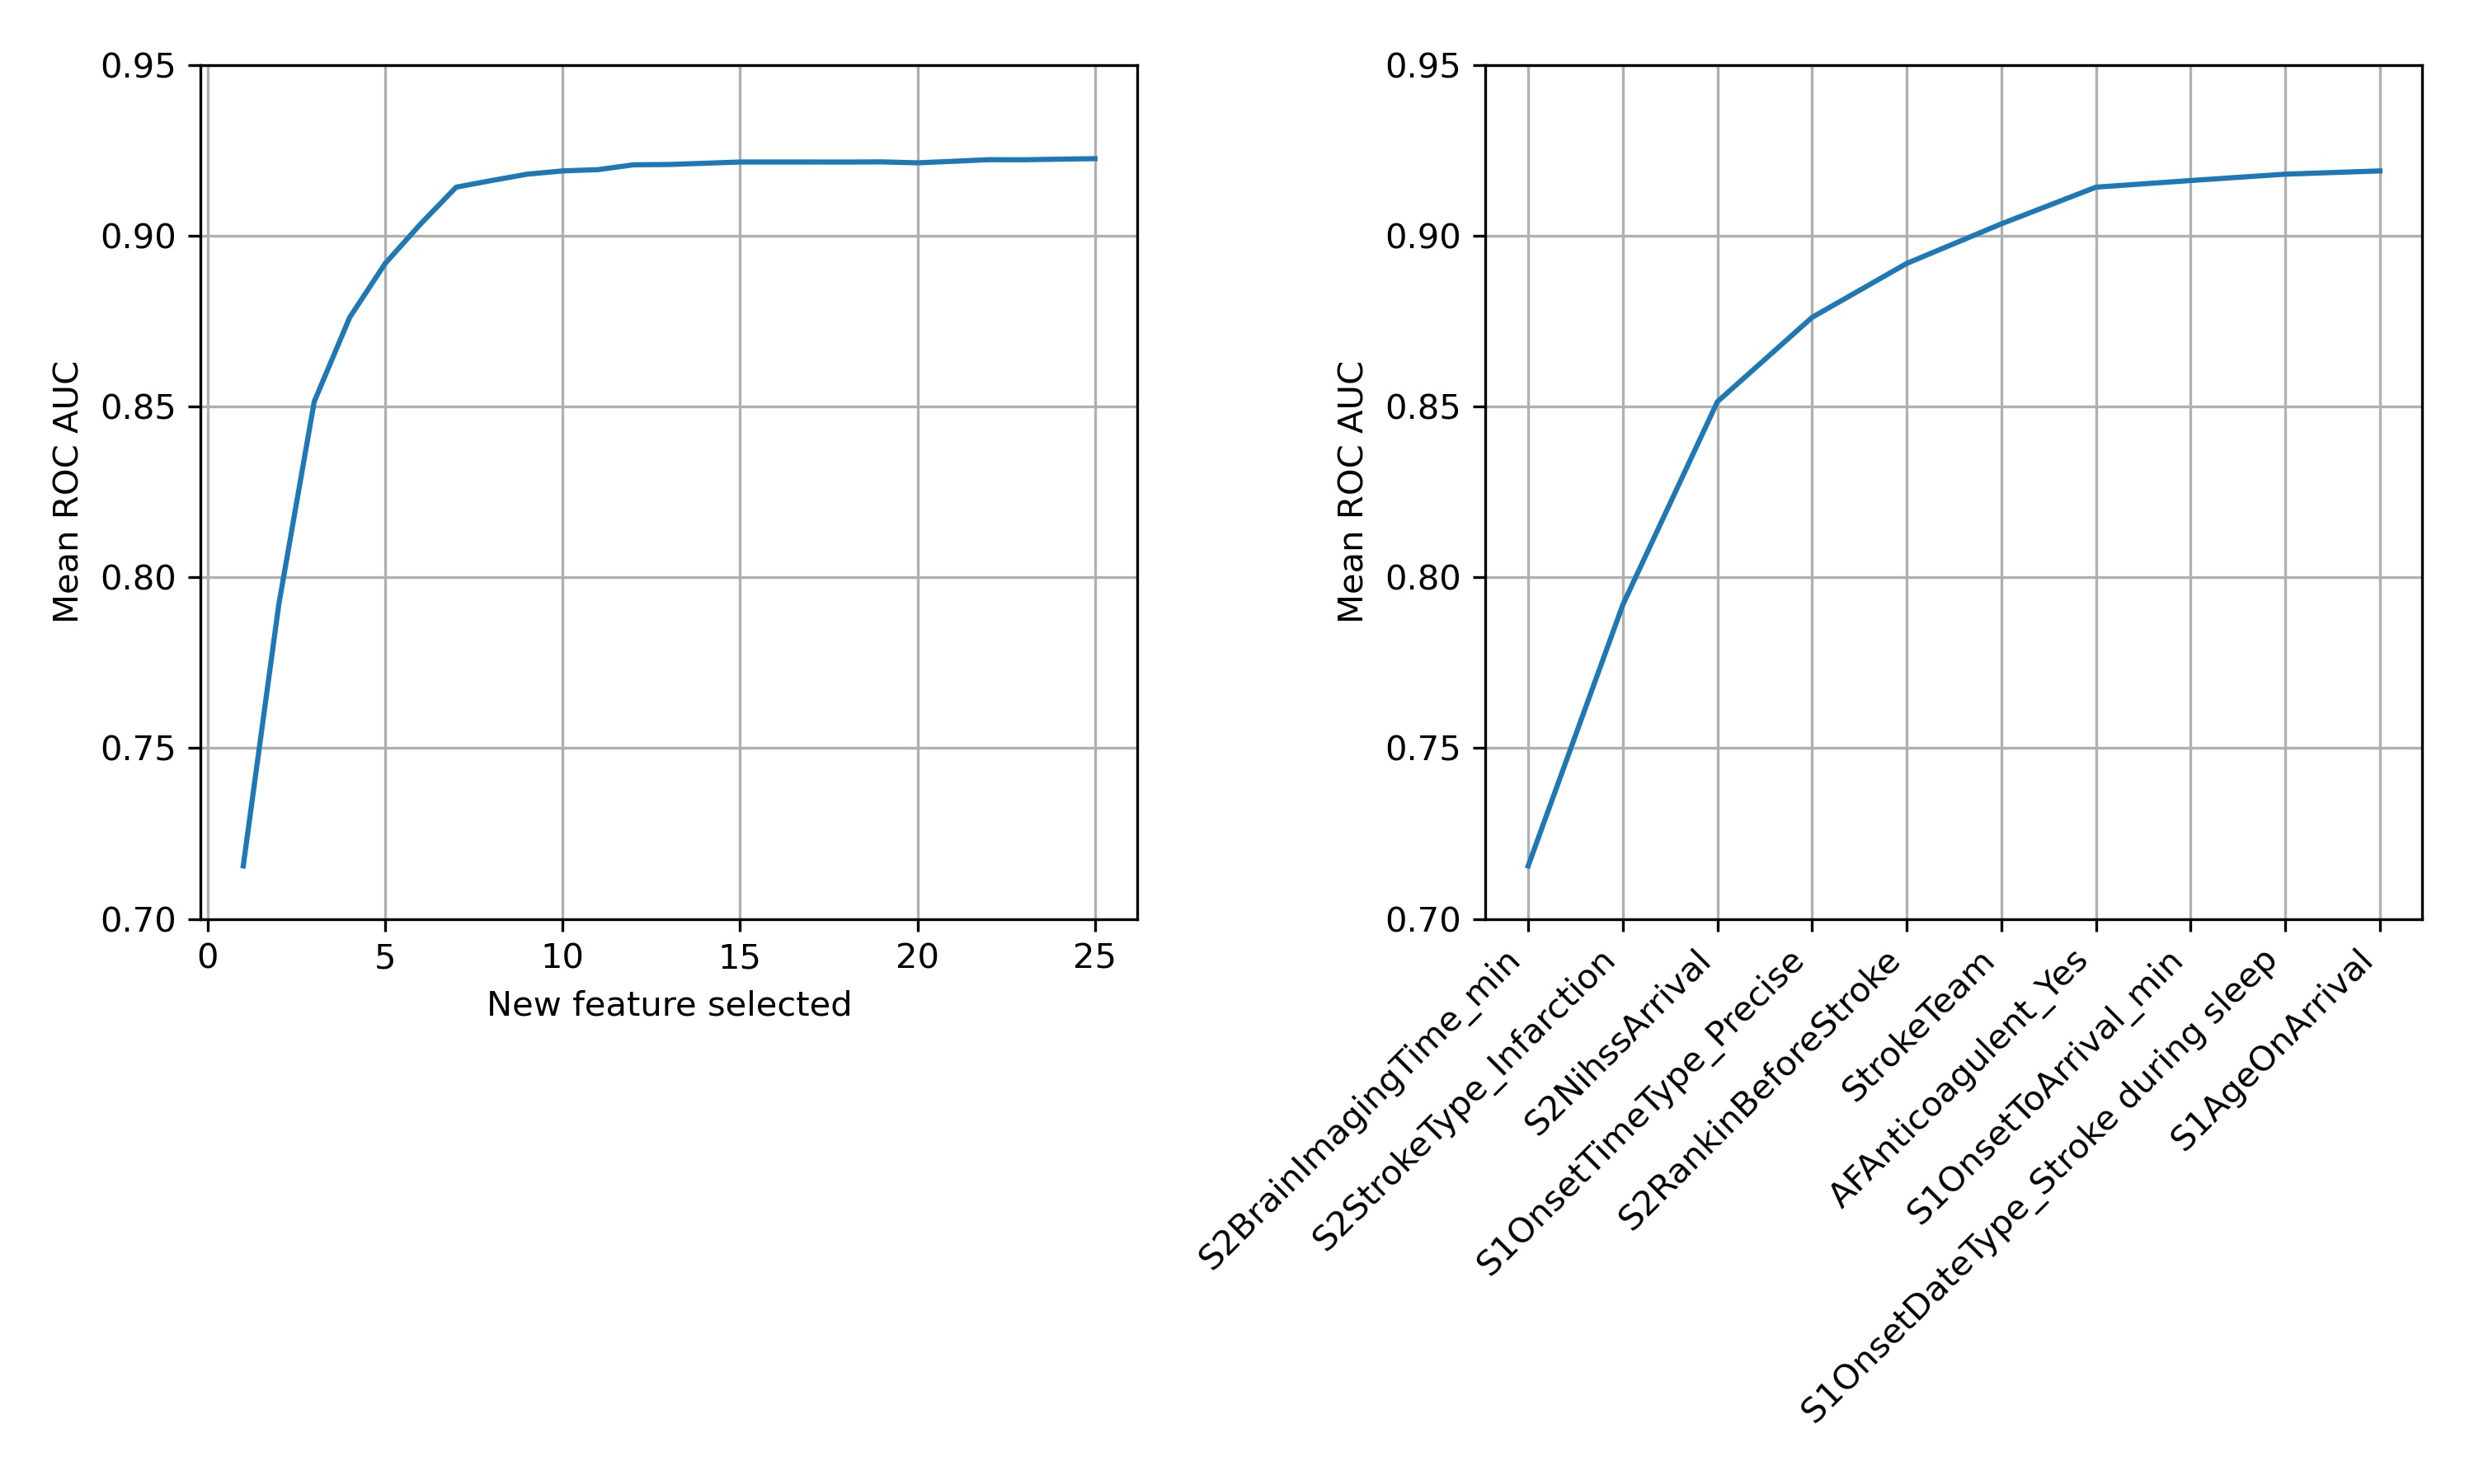
\includegraphics[width=1\textwidth]{./images/01_feature_selection}
\caption{The effect of progressively selecting more features on ROC AUC. Left: ROC AUC with selection of up to 25 features. Right: The first 10 selected features and the resulting ROC AUC.}
\label{fig:feature_selection}
\end{figure}

All results from this point forward will use the 10 feature model.

%%%%%%%%%%%%%%%%%%%%%%%%%%%%%%%%%%%%%%%%%%%%%%%%%%%%%%%%%%%%%%%%%%%%%%%%%%%%%%%%%%%%%%%

\subsection{Model accuracy}

The model was validated using stratified k-fold validation (k=5).





